\documentclass{article}
\usepackage{geometry}
\usepackage{tzplot}
\geometry{paperwidth=5.31in, paperheight=3in, left=15mm, right=15mm, bottom=10mm}
\pagenumbering{gobble}
\usepackage{tzplot}
\usepackage{amsmath}
\usepackage[utopia]{mathdesign}
\usepackage{multicol}
\begin{document}

\Large

\vspace*{\fill}
\begin{center}
{\LARGE{
\texttt{Quadratic Equation}
}}
\end{center}
\vspace*{\fill}


\pagebreak
\[
\textbf{Graph of quadratic function}
\]
\begin{enumerate}
\item $ f(x)=ax^2 + bx + c 
 \quad \left( a, b, c \in \text{R \& $a\neq0$} \right)$
 
 \pagebreak 
 \begin{enumerate}
 \item Step-I
	\begin{itemize}
	\item Case-I, $\quad a>0$
	\pagebreak
	\item Case-II, $\quad a<0$
	\end{itemize}
	\pagebreak
	\item Step-II
	\begin{itemize}
	\item $\quad D>0$
	\pagebreak
	\item $\quad D<0$
	\pagebreak
	\item $\quad D=0$
	\end{itemize}
\end{enumerate}	 
 $~$
 \pagebreak

\item Vertex of quadratic function
\begin{multicols}{2}
\begin{center}
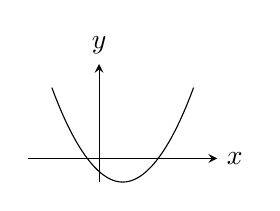
\begin{tikzpicture}[scale=0.3]
	\tzaxes(-3, -1)(5, 4){$x$}{$y$}
	\tzparabola(-2, 3)(1, -1)(4, 3)
\end{tikzpicture}
\end{center}
\begin{center}
\begin{tikzpicture}[scale=0.3]
	\tzaxes(-3, -1)(5, 4){$x$}{$y$}
	\tzparabola(-1, 3)(1, 1)(3, 3)
\end{tikzpicture}
\end{center}
\begin{center}
\begin{tikzpicture}[scale=0.3]
	\tzaxes(-3, -2)(5, 2){$x$}{$y$}
	\tzparabola(-1, -2)(1, 0)(3, -2)
\end{tikzpicture}
\end{center}
\begin{center}
\begin{tikzpicture}[scale=0.3]
	\tzaxes(-3, -1)(5, 4){$x$}{$y$}
	\tzparabola(-2, -1)(1, 3)(4, -1)
\end{tikzpicture}
\end{center}
\end{multicols}

\pagebreak 
\vspace*{\fill}
\pagebreak $~$
\vspace*{\fill}
\pagebreak $~$
\vspace*{\fill}
\pagebreak $~$
\vspace*{\fill}

\end{enumerate}


\end{document}
